\documentclass{beamer}
% \documentclass[handout]{beamer}
\usepackage{cuhkbeamer}


\title[Short title]{Your Title}
\subtitle{Your Subtitle}
\author[Short name]{
    Your name \\
    \vspace{0.1in}
    \footnotesize{Email: XXX@xxx.cuhk.edu.hk} \\
    \footnotesize{Office: Pavilion of Harmony, CUHK}}
\institute[CUHK]{The Chinese University of Hong Kong}
\date{\today}


\begin{document}


% Title page
\frame[plain]{\maketitle}

% Outline
\begin{frame}{Outline}
    \label{outline}
    \tableofcontents{}
\end{frame}

% Text, Lists, Tables and Figures
\slidesection{Text, Lists, Tables and Figures}

\begin{frame}{Text and lists}
    Lorem ipsum dolor sit amet, consectetur adipiscing elit, sed do eiusmod tempor incididunt ut labore et dolore magna aliqua. \pause
    \begin{itemize}
      \item Time-dependent Schr\"{o}dinger's equation: $$i \hbar \frac{\partial}{\partial t}\lvert\Psi(t)\rangle = \hat H \lvert\Psi(t)\rangle$$ \pause
      \item Mathematically, a function $f(x)$ is linear iff $f(u+v)=f(u)+f(v)$ and $f(cu)=cf(u)$. \pause
    \end{itemize} \pause
    \vspace{0.1in}
    Duis aute irure dolor in reprehenderit in voluptate velit esse cillum dolore eu fugiat nulla pariatur. \pause
\end{frame}

\begin{frame}{Figure}
    Excepteur sint occaecat cupidatat non proident, sunt in culpa qui officia deserunt mollit anim id est laborum.
    \begin{figure}
        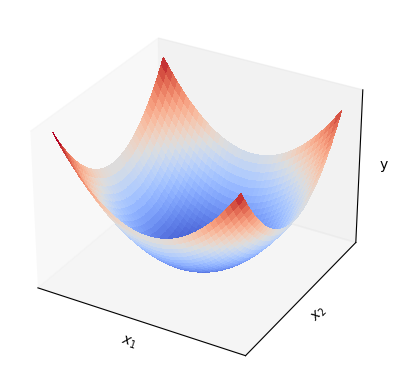
\includegraphics[width=0.5\textwidth]{images/convex_surface.png}
    \end{figure}
\end{frame}

\begin{frame}{Table}
    Ut enim ad minim veniam, quis nostrud exercitation ullamco laboris nisi ut aliquip ex ea commodo consequat.
    \vspace{0.4in}
    \begin{table}
        \footnotesize
        \begin{tabular}{l | l | l}
        Index & Areas ($m^2$) & Rent (HKD) \\
        \hline \hline
        1 & 40 & 134072 \\ 
        2 & 92 & 182241 \\
        3 & 37 & 134731 \\
        4 & 124 & 204325 \\
        5 & 88 & 187375 \\
        ... & ... & ...
        \end{tabular}
    \end{table}
\end{frame}

% Columns, Code, Links and Footnote
\slidesection{Columns, Code, Links and Footnote}

\begin{frame}{Columns}
    \begin{columns}
        \column{0.5\textwidth}
        \onslide<1->\begin{enumerate}
            \item Sed ut perspiciatis unde omnis iste natus error sit voluptatem accusantium doloremque laudantium.
            \item Nemo enim ipsam voluptatem quia voluptas sit aspernatur aut odit aut fugit.
            \item Totam rem aperiam, eaque ipsa quae ab illo inventore veritatis et quasi architecto beatae vitae dicta sunt explicabo.
        \end{enumerate}
        \column{0.5\textwidth}
        \onslide<2->\begin{figure}
            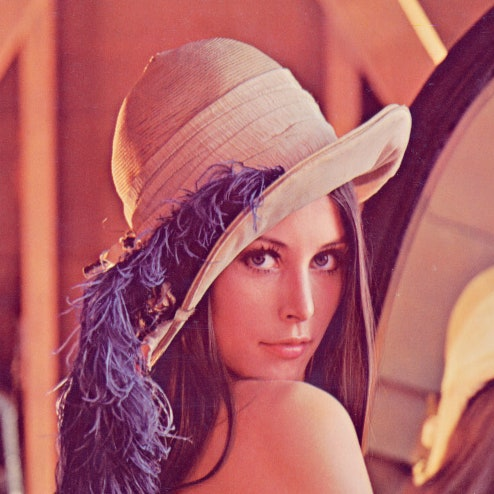
\includegraphics[width=0.8\textwidth]{images/lenna.jpg}
        \end{figure}
    \end{columns}
\end{frame}

\begin{frame}{Code}
    \begin{algorithm}[H]
        \caption{An algorithm with caption}
        \begin{algorithmic}
            \Require $n \geq 0$
            \Ensure $y = x^n$
            \State $y \gets 1$
            \State $X \gets x$
            \State $N \gets n$
            \While{$N \neq 0$}
            \If{$N$ is even}
                \State $X \gets X \times X$
                \State $N \gets \frac{N}{2}$  \Comment{This is a comment}
            \ElsIf{$N$ is odd}
                \State $y \gets y \times X$
                \State $N \gets N - 1$
            \EndIf
            \EndWhile
        \end{algorithmic}
    \end{algorithm}
\end{frame}

\begin{frame}{Links}
    \begin{itemize}
        \item \href{https://en.wikipedia.org/wiki/Beamer_(LaTeX)}{Beamer (LaTex) - Wikipedia}
        \item Please refer to page \ref{outline}.
        \item \url{https://en.wikipedia.org/wiki/Beamer_(LaTeX)}
    \end{itemize}
\end{frame}

\begin{frame}{Footnote}
    \begin{itemize}
        \item \emphacolor{Beamer} is a \LaTeX~~document class for creating presentation slides, with a wide range of templates and a set of features for making slideshow effects. It supports pdfLaTeX, LaTeX + dvips, LuaLaTeX and XeLaTeX. The name is taken from the German word ``Beamer'' as a pseudo-anglicism for ``video projector''. \footnote{\href{https://en.wikipedia.org/wiki/Beamer_(LaTeX)}{https://en.wikipedia.org/wiki/Beamer\_(LaTeX)}}
    \end{itemize}
\end{frame}

% Equations and Blocks
\slidesection{Equations and Blocks}

\begin{frame}{Example}
    \begin{example}
        Lorem ipsum dolor sit amet, consectetur adipiscing elit, sed do eiusmod tempor incididunt ut labore et dolore magna aliqua. Ut enim ad minim veniam, quis nostrud exercitation ullamco laboris nisi ut aliquip ex ea commodo consequat.
    \end{example}
\end{frame}

\begin{frame}{Theorem}
    \begin{theorem}
        $\mathbf{X}^T\mathbf{X}$ is invertible $\iff \mathbf{X}$ has linearly independent columns.
    \end{theorem}\pause
    \vspace{0.2in}
    \begin{proof}
        Firstly, note that $\mathbf{X}^T\mathbf{X} \in \mathbf{R}^{n \times n}$. We denote $N(\mathbf{X})$ as the kernel (nullspace) of $\mathbf{X}$, and $R(\mathbf{X})$ as the range (column space) of $\mathbf{X}$. \\
        We prove $\mathbf{X}^T\mathbf{X}$ and $\mathbf{X}$ share the same kernel such that once $N(\mathbf{X}) = 0$, $N(\mathbf{X}^T\mathbf{X}) = 0$ and vice versa.
    \end{proof}
\end{frame}

\begin{frame}{Proof}
    \begin{proof}
        1) Prove $N(\mathbf{X}) \subset N(\mathbf{X}^T\mathbf{X})$ \\
        $\forall v \in N(\mathbf{X})$, $\mathbf{X}^T\mathbf{X}v = \mathbf{X}^T0 = 0$ $\implies v \in N(\mathbf{X}^T\mathbf{X}) \implies N(\mathbf{X}) \subset N(\mathbf{X}^T\mathbf{X})$. \\ \pause
        
        \vspace{0.2in}
        2) Prove $N(\mathbf{X}^T\mathbf{X}) \subset N(\mathbf{X})$ \\
        $\forall v\neq 0 \in N(\mathbf{X}^T\mathbf{X})$, $\mathbf{X}^T\mathbf{X}v = 0$ $\implies$ $v \in N(\mathbf{X}^T)$ or $\mathbf{X}v \in N(\mathbf{X}^T)$. However, we have $R(\mathbf{X}) \perp N(\mathbf{X}^T)$ and $\mathbf{X}v \in R(\mathbf{X})$, $\implies \mathbf{X}v \perp N(\mathbf{X}^T) \implies \mathbf{X}v \notin N(\mathbf{X}^T) \implies v \in N(\mathbf{X}^T)$
        $\implies N(\mathbf{X}^T\mathbf{X}) \subset N(\mathbf{X})$ \\ \pause
        
        \vspace{0.2in}
        1), 2) $\implies \mathemphacolor{N(\mathbf{X}^T\mathbf{X}) = N(\mathbf{X})}$
    \end{proof}
\end{frame}

% References
\slidesection{References}

\begin{frame}{References}
    \begin{itemize}
        \item \href{https://www.overleaf.com/learn}{Overleaf Documentation}
        \item \href{https://www.overleaf.com/learn/latex/Learn_LaTeX_in_30_minutes}{Learn LaTeX in 30 Minutes}
        \item \href{https://www.overleaf.com/learn/latex/Beamer}{LaTeX Beamer - Overleaf}
        \item \href{https://www.overleaf.com/learn/latex/Beamer_Presentations:_A_Tutorial_for_Beginners_(Part_1)\%E2\%80\%94Getting_Started}{Beamer Presentations: A Tutorial for Beginners}
    \end{itemize}
\end{frame}


\end{document}